\documentclass[final,hyperref={pdfpagelabels=false}]{beamer}
\usepackage{grffile}
\mode<presentation>{\usetheme{I6pd2}}
\usepackage[brazil]{babel}
\usepackage[utf8]{inputenc}
\usepackage{amsmath,amsthm, amssymb, latexsym}
\usepackage{graphicx}
\boldmath
\usepackage[orientation=portrait,size=a0,scale=1.4,debug]{beamerposter}
\usepackage{nicealgo}
\usepackage{array,booktabs,tabularx}
\newcolumntype{Z}{>{\centering\arraybackslash}X}
\newcommand{\pphantom}{\textcolor{ta8aluminium}}

\setbeamertemplate{caption}[numbered]

\listfiles

%%%%%%%%%%%%%%%%%%%%%%%%%%%%%%%%%%%%%%%%%%%%%%%%%%%%%%%%%%%%%%%%%%%%%%%%%%%%%%%%%%%%%%

\title{\Huge O título do seu trabalho deve ser escrito aqui}
\author{\Large $^1$Autor da Filiação 1, $^2$Autor da Filiação 2, etc}
\institute[UNESP, ETC]{$^1$Universidade Estadual Paulista - Brasil, $^2$Filiação 2 - Brasil} 

%%%%%%%%%%%%%%%%%%%%%%%%%%%%%%%%%%%%%%%%%%%%%%%%%%%%%%%%%%%%%%%%%%%%%%%%%%%%%%%%%%%%%%
\newlength{\columnheight}
\setlength{\columnheight}{105cm}


%%%%%%%%%%%%%%%%%%%%%%%%%%%%%%%%%%%%%%%%%%%%%%%%%%%%%%%%%%%%%%%%%%%%%%%%%%%%%%%%%%%%%%
\begin{document}
\begin{frame}
	\begin{columns}
		% ---------------------------------------------------------%
		% Set up a column 
		\begin{column}{.45\textwidth}
			\begin{beamercolorbox}[center,wd=\textwidth]{postercolumn}
				\begin{minipage}[T]{.95\textwidth}  % tweaks the width, makes a new \textwidth
					\parbox[t][\columnheight]{\textwidth}{ % must be some better way to set the the height, width and textwidth simultaneously
						% Since all columns are the same length, it is all nice and tidy.  You have to get the height empirically
						% ---------------------------------------------------------%
						% fill each column with content        
						
						\begin{block}
							{\vspace{-6pt} \large I -- Seção}
							Espaço para a seção 1.          
						\end{block}
						%\vfill
						\vspace*{14pt}
						
						\begin{block}{\vspace{-6pt} \large II -- Seção}
							\begin{itemize}
								
								{\small \item LaTeX normal funciona aqui.}
								
								
							\end{itemize}
						\end{block}
						
						\vspace*{14pt}
						
						\begin{block}{\vspace{-6pt} \large II.A -- Subseção}
						\end{block}
						
						\begin{block}{\vspace{-6pt} \large III -- Figuras}
							
							\begin{figure}[h]
								\centering
								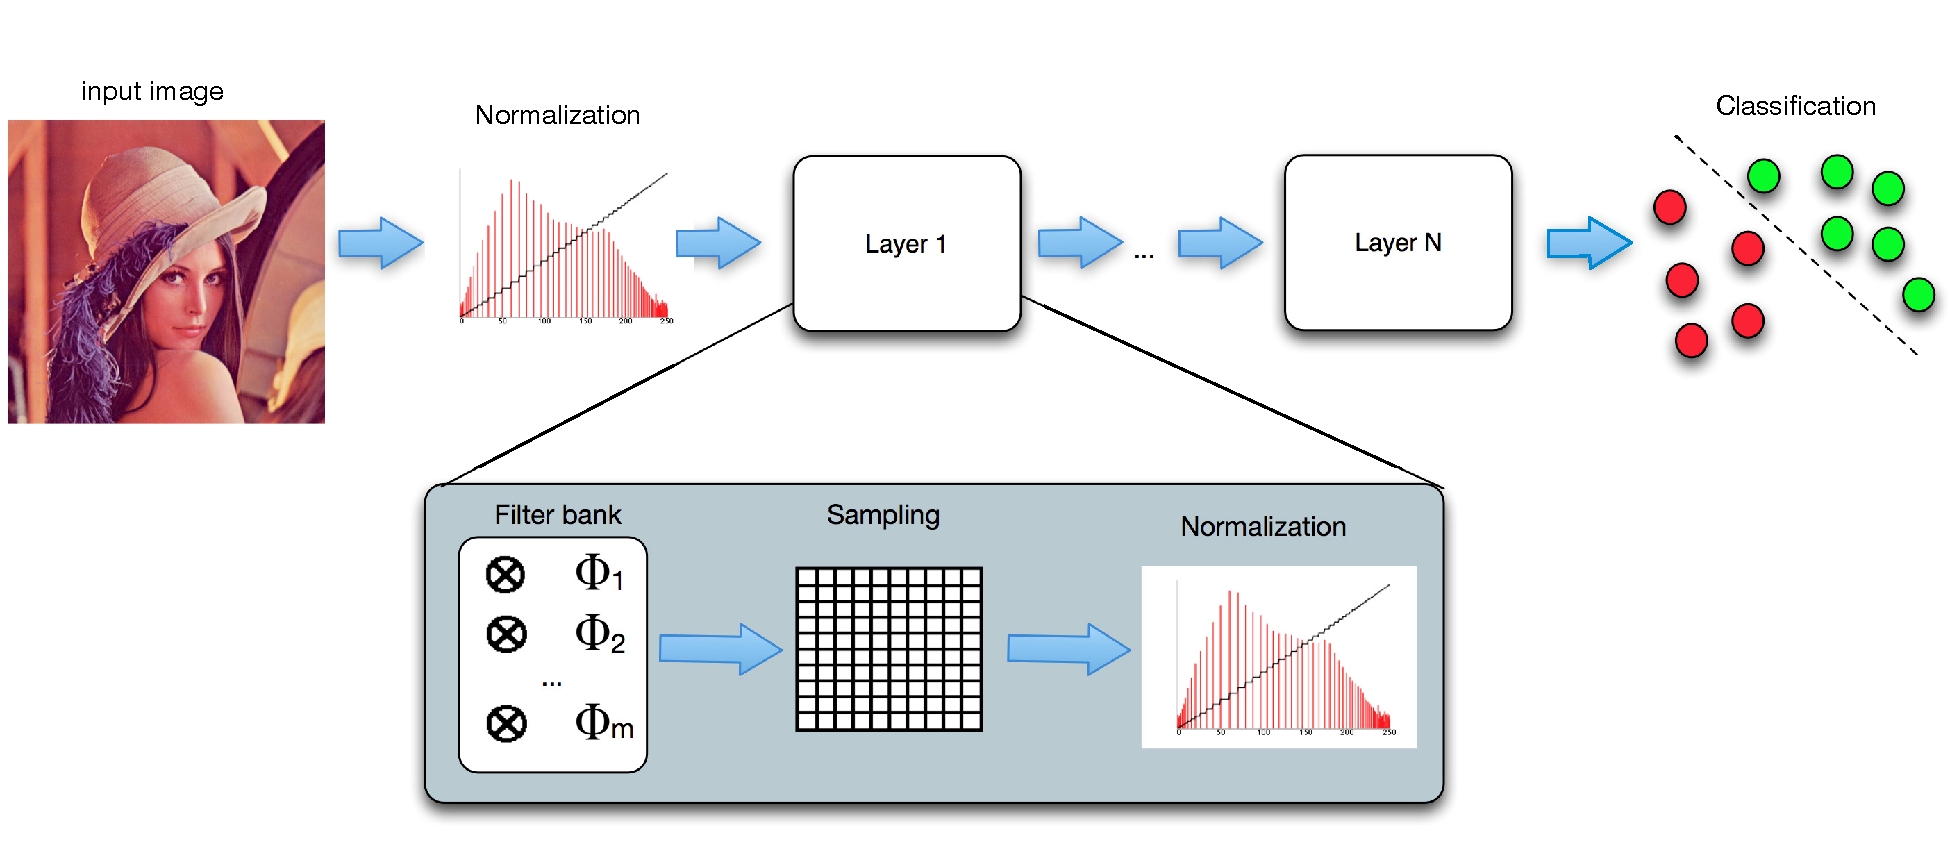
\includegraphics[scale=1.00]{figs/deep.pdf}
								\caption{\small Legenda.}
								\label{f.deep_architecture}
							\end{figure}
							
						\end{block}
					}
				\end{minipage}
			\end{beamercolorbox}
		\end{column}
		% ---------------------------------------------------------%
		% end the column
		
		% ---------------------------------------------------------%
		% Set up a column 
		\begin{column}{.54\textwidth}
			\begin{beamercolorbox}[center,wd=\textwidth]{postercolumn}
				\begin{minipage}[T]{.95\textwidth} % tweaks the width, makes a new \textwidth
					\parbox[t][\columnheight]{\textwidth}{ % must be some better way to set the the height, width and textwidth simultaneously
						% Since all columns are the same length, it is all nice and tidy.  You have to get the height empirically
						% ---------------------------------------------------------%						
						\begin{block}{\vspace{-6pt} \large IV -- Tabelas}
							
							{\small \begin{table}[h]
								\centering
								\caption{\footnotesize Legenda.}
								\scalebox{0.70}{
									\begin{tabular}{|c|c|} \hline
										Technique & Parameters                               \\ \hline\hline
										HS        & $HMCR=0.7$, $PAR=0.5$, $\varrho=0.1$     \\ \hline
										IHS       & $HMCR=0.7$, $PAR_{MIN}=0.0$              \\ 
										          & $PAR_{MAX}=1.0$, $\varrho_{MIN}=0.0$     \\ 
										          & $\varrho_{MAX}=0.1$                      \\ \hline
										GHS       & $HMCR=0.7$, $PAR_{MIN}=0.1$              \\ 
										          & $PAR_{MAX}=1.0$                          \\ \hline
										SGHS      & $HMCR_{m}=0.98$, $PAR_{m}=0.9$           \\ 
										          & $\varrho_{MIN}=0.0$, $\varrho_{MAX}=0.1$ \\ 
										          & $LP = 100$                               \\ \hline
									\end{tabular}
								}
								\label{t.parameters}
								\end{table}}
							
							\vspace*{14pt}
							
							{\small \begin{table}
								\parbox{.45\linewidth}{
									\caption{\footnotesize Legenda.}
									\centering
									\scalebox{0.70}{
										\begin{tabular}{|c|c|c|c|} \hline
											Technique     & Final Accuracy            & \#calls      \\ 
											              & (test set)                &              \\\hline\hline
											Caffe         & 99.07\%$\pm$0.03          & 1            \\ \hline
											RS            & 98.70\%$\pm$0.56          & 1            \\ \hline
											HS            & 99.23\%$\pm$0.04          & 265          \\ \hline
											\textbf{IHS}  & \textbf{99.24\%$\pm$0.03} & \textbf{265} \\ \hline
											\textbf{GHS}  & \textbf{99.24\%$\pm$0.08} & \textbf{265} \\ \hline
											\textbf{SGHS} & \textbf{99.29\%$\pm$0.06} & \textbf{265} \\ \hline
										\end{tabular}
								}}
								\hfill
								\parbox{.45\linewidth}{
									\caption{\footnotesize Legenda.}
									\centering
									\scalebox{0.70}{
										\begin{tabular}{|c|c|c|c|} \hline
											Technique     & Final Accuracy            & \#calls      \\ 
											              & (test set)                &              \\\hline\hline
											Caffe         & 71.51\%$\pm$0.77          & 1            \\ \hline
											RS            & 66.97\%$\pm$1.39          & 1            \\ \hline
											\textbf{HS}   & \textbf{72.28\%$\pm$0.37} & \textbf{265} \\ \hline
											IHS           & 71.54\%$\pm$0.09          & 265          \\ \hline
											GHS           & 71.86\%$\pm$0.10          & 265          \\ \hline
											\textbf{SGHS} & \textbf{72.43\%$\pm$0.19} & \textbf{265} \\ \hline
										\end{tabular}
								}}
								\end{table}}
							
							\vspace*{14pt}
							
							\begin{itemize}
								
								{\small \item Citação~\cite{jia2014caffe}.}
								
							\end{itemize}
							
							
						\end{block}
						
						\vspace*{8pt}
						
						\begin{block}{\vspace{-6pt} \large V -- Seção}
						\end{block}
						
						% ---------------------------------------------------------%
						\vspace*{8pt}
						
						\begin{block}{\vspace{-6pt} \large Agradecimentos}
							{\small Os autores agradecem...}
						\end{block}	
						
						\vspace*{8pt}
						
						\begin{block}{\vspace{-6pt} \large Referências}
							{\tiny
								\bibliographystyle{abbrv}
								\bibliography{references}}
						\end{block}
						
						\vspace*{8pt}
						
						
						
					}
					% ---------------------------------------------------------%
					% end the column
				\end{minipage}
			\end{beamercolorbox}
		\end{column}
		% ---------------------------------------------------------%
		% end the column
	\end{columns}
\end{frame}
\end{document}